\chapter{Preliminaries}
\label{chap:preliminaries}

This section serves as a technical primer to all the security related software solutions that are employed in this paper. An in-depth discussion of these topics is considered out of scope. First, the main characteristics of microcontrollers are presented. Second, the concept of role-based access control is introduced. Third, the reader is familiarised with public key cryptography, and what sets it apart from symmetric cryptography. Fourth, we will take a look at how secret keys (asymmetric or symmetric) are established between two parties. Fifth, we will explain how public key cryptography can be used in the context of authentication. Sixth, the concept of hashing and why it i useful is explained. Seventh, the concept of security level is concisely explained. The last chapter of this section gives an overview of all the specific implementations that were selected by the researchers of this paper, as well as motivating these decisions. The reader should keep in mind that the selection of algorithms and systems selected here is far from comprehensive, only those that are relevant to the solution presented in this paper (see section \ref{sec:solution}) are discussed. 


\section{ECU Microcontrollers}
\label{sec:microcontrollers}

As discussed before, an ECU is an embedded computer that is designed to perform a specific function. The core of any ECU is a small computer on an integrated circuit called a microcontroller. A microcontroller consists of one or more central processing units (CPUs)  along with memory and programmable input/output peripherals. There a couple of characteristics of microcontrollers that are touched upon in the course of this paper, so a description of these characteristics is given next:

\begin{itemize}
	\item \textbf{Word size:} The word size of a microcontroller (or any computer for that matter) is the natural unit of data used by a particular processor. A word is a fixed-sized piece of data handled as a single unit by the instruction set or the hardware of the processor. The number of bits in a word, called the word size, is an important characteristic of any microcontroller. Within the context of ECU's, word sizes of 8 bits (e.g. driver information), 16 bits (e.g. vehicle control) and 32 bits (power train) are most common.\cite{ECU}
	
	\item \textbf{Clock rate:} The clock rate of a CPU refers to the rate at which it processes words of data. it is used as an indicator of the processor's speed. It is measured in clock cycles per second or hertz (Hz). 
	
	\item \textbf{Memory:} There are two basic types of memory: data memory and program memory.
	\begin{itemize}
		\item \textbf{Data Memory}: Data memory is where variables and all intermediate calculations are stored by the CPU. It is generally implemented by RAM \footnote{random access memory (RAM) is a type of memory where individual data can be read or written in almost the same amount of time irrespective of the physical location of data inside the memory.}. This data is often volatile, meaning the data is lost when power is removed.
		
		\item \textbf{Program memory}: Program memory is where the application is stored, i.e. the code itself. This type of memory is implemented using non-volatile storage technologies like ROM \footnote{Read-only memory (ROM) is a type of non-volatile memory where the data stored can not be modified (or where it is considered very difficult to do so).}, EPROM\footnote{erasable programmable read-only memory (EPROM) is a non-volatile type of memory that can be erased (by exposing the chip the ultraviolet light) and reprogrammed.}, EEPROM\footnote{Electrically erasable programmable read-only Memory (EEPROM) is a type of non-volatile memory that can be erased and reprogrammed electronically.} or Flash Memory\footnote{Flash memory is type of EEPROM  that can be electrically erased and reprogrammed much faster than regular EEPROM chips by using large erase blocks.}.
	\end{itemize}
	
	\item \textbf{Serial Communications Interfaces:} Serial communications is a way of communication in computer networks where bits are transmitted one bit at a time (e.g. CAN). This is in contrast to parallel communications where a link is used with several parallel channels, allowing multiple bits to be sent at the same time (e.g. USB). Most microcontrollers offer dedicated hardware allowing for easy communication with other devices (e.g. CAN controller).
	
	\item \textbf{Others:} Most microcontrollers offer various other hardware like: a timer, an analog-to-digital convertor (ADC) that allows for an analog signal (like the output of a sensor) to be transformed into a digital signal, a clock generator, etc.
\end{itemize}

\section{Role-Base Access Control}
\label{sec:RBAC}

Role-based access control (RBAC) is a well-defined way of restricting system access to authorized users. It especially useful in large enterprises where roles are created for various job functions. Each role is assigned the necessary permissions to interact with a secured system (e.g. the company database, the local private network, development software, etc). The idea is that a worker is assigned a role based on what he/she requires to do his/her job, and nothing more. This way it is avoided that workers are granted permissions they do not require. There are two basic types of RBAC\cite{wiki:RBAC}:

\begin{itemize}
	\item \textbf{Mandatory Access Control:} In a system where mandatory access control (MAC) is a enforced, only the administrator of the system is able to create and assign roles. This is done by defining a security policy that users are unable to override or alter. The administrator of the system is called the security policy administrator.
	
	\item \textbf{Discretionary Access Control:} When discretionary access control (DAC) is enforced, it is up to the users themselves to make policy decisions and/or assign security attributes.
\end{itemize}


\section{Public Key Cryptography}
\label{sec:PKC}

\paragraph{Cryptography} The primary goal of cryptography in general is to allow for secure communication between two parties. This means that protocols are designed that prevent third parties or the public in general from reading private messages. This is done by encrypting the message, which consists of converting the information from a readable state to apparent nonsense. Only the intended recipient should be able to restore the information to it's original form, which is called decryption. To allow for this to work, the procedure of encryption and decryption should only be possible by the sender and the receiver respectively. Generally this procedure consists of two parts. First, there is the cypher, which is the algorithm that does the actual conversion. Second, there's the secret key, which is used by the cipher together with the input (plaintext) to create the encrypted output (ciphertext). The main advantage of this architecture is that the chosen cipher can be made public, as long as the key is kept secret. The receiver of the secret message, who is in possession of the same secret key, runs the same cipher in reverse with the secret key and the ciphertext as inputs, yielding the original plaintext.\cite{wiki:Cryptography}

\paragraph{Symmetric vs Asymmetric}The procedure outlined above is called symmetric key cryptography since both parties are in possession of the same secret key. The disadvantage here is that these keys need to be securely exchanged beforehand (e.g. via a secure channel) to allow for secure communications. Asymmetric (or public key) cryptography offers a solution to this problem. In this case a key pair is created where each one serves a specific function. The first one is called the private key, which is meant to be kept secret at all times by the owner. The second one is called the public key, which is disseminated widely to the public. The idea is that if someone wants to send an encrypted message to the owner of the private key, he/she looks up the corresponding public key (generally found online), uses it to encrypt a message, and sends this message to the owner. Since only the owner is in possession of the corresponding private key, he/she is able to decrypt the message.

\section{Key Exchange} 
\label{sec:key_exchange}

The specifications of symmetric and asymmetric encryption are sound. However they both rely on both parties being in possession of the right key. In the case of asymmetric encryption this is easy: The owner generates a new public/private key pair, stores the private key in a safe location, and distributes the corresponding public key on the internet. Anyone wanting to securely communicate with the owner only has to look up the corresponding public key. This procedure does not apply to symmetric encryption however, since only the sender and receiver should be in possession of the secret key. One way of safely distributing the key is to use a secure communications channel. Examples of this are: a text message, a phone call, physically handing over the key, sending a letter, etc. It is clear however that in most situations this method simply will not do, since it requires significant effort before a secure communication session can be established. Two more realistic alternatives exist: using asymmetric keys to establish a session key and key exchange algorithms. Both will be discussed in turn next.

\paragraph{Session Keys} In this solution the free distribution of public keys is leveraged to establish a new temporary shared key, also called a session key. If Alice has an asymmetric key pair already established, and Bob wishes to establish a shared secret key with Alice. Bob only has to look up Alice's public key, generate a new session key, encrypt the new session key using Bob's public key and send it to Alice. Alice can then decrypt the session key using her private key. In the end both parties are in possession of the new session key, and a secure communication can be established. Now, the reader might wonder why it is necessary to establish a session key, since secure communications could also be performed using asymmetric keys (granted they both have an asymmetric key pair)? Well, this is mainly due to performance. Asymmetric encryption requires significantly longer keys to guarantee the same level of security, and the corresponding procedures (e.g. encryption, decryption, signing, etc.) take significantly longer to perform. Therefore, it is often beneficial to establish a session key and using these, instead of repeatedly using asymmetric keys.

\paragraph{Key Exchange Algorithms} Key exchange algorithms allow two parties that have no prior knowledge of each other to establish a shared secret key over an insecure channel. The most famous example of such an algorithm is the Diffie-Hellman key exchange method (for more information on Diffie-Hellman see \cite{wiki:DH}). These algorithms typically rely on computationally hard to solve mathematical problems such as the discrete logarithm.

\section{Authentication} 
\label{sec:authentication}

Besides protecting messages from being read by a third party, the recipient of the message might also want certainty on who sent it in the first place, as well as knowing that the message has not been tampered with. In other words the recipient wants to guarantee the integrity of the message, as well as to authenticate the sender. Fortunately asymmetric and symmetric cryptography offer solutions in the form of digital signatures and message authentication codes respectively. Before going into this however, it is necessary to first take a look at hash functions.

\subsection{Hash functions} 
\label{subsec:hash_functions}

A hash function is used to map data of arbitrary size to data of a fixed size. The values returned by a hash function are called hash values, hash codes, digests, or simply hashes\footnote{We will be using the term hash values when referring to the output of a hash function}. For a hash function to be useful in cryptography (also called a cryptographic hash function) it has to possess the following properties\cite{wiki:Hash}:

\begin{itemize}
	\item The same message always results in the same hash value.
	\item The hash function does not take long to perform.
	\item It is infeasible to reconstruct the original message from the hash value.
	\item Two similar messages have widely varying hash values.
	\item it is infeasible to find two different messages with the same hash value.
\end{itemize}

\subsection{Digital Signatures} 
\label{subsec:digital_signature}

A digital signature is used to verify the authenticity of digital messages. The principle is simple: If Alice wants to send an authenticated message to Bob, she will first sign the message using her private key. She then sends the message, together with the generated signature to Bob. Bob can then check the authenticity of the message by verifying the signature using Alice's public key. If the verification was successful Bob can safely assume 2 things: the message was sent by Alice (since only she is in possession of the corresponding private key) and the message was not tampered with in transit (since in that case the signature would no longer match the message, resulting in a failed verification) 2 additional algorithms are required: a signing algorithm and a signature verification algorithm. Ideally the signing algorithm would produce a signature of the same size, regardless of the size of the original message. This is where cryptographic hash functions come in, since they possess this property. Generally the message will first be hashed to a fixed size, before being processed by the signing algorithm. Besides guaranteeing a fixed sized output, this also improves the overall efficiency.\cite{wiki:DigitalSignature}

\subsection{MAC's} 
\label{subsec:MAC}
a message authentication code (MAC) serves the same function as a digital signature algorithm. Namely, guaranteeing the authenticity and integrity of a transmitted message. The main difference is that MAC's are based on symmetric keys rather than asymmetric keys. 

\section{Authenticated Key Agreement}
\label{sec:AK}

As will become apparent in section \ref{sec:authentication_procedure} it is generally advised to combine authentication and shared secret establishment into a single procedure. This is called authenticated key agreement (AK). In AK systems both parties are mutually authenticated while a shared secret is established. It is only assured that both parties are able to generate the shared secret, not that this secret was actually computed. A protocol that also guarantee to both parties that the other party actually computed the secret is called authenticated key agreement with key confirmation (AKC).\cite{Blake-Wilson}

\section{Security Level}
\label{sec:security_level}

The security level of a cryptographic primitive (e.g. a hash function, a key, a cipher) refers to the difficulty for any attacker to break it. The security level is usually expressed in bits, where $n$-bit security means that an attacker would have to perform (at least) $2^n$ operations to effectively crack the cryptographic primitive. It is very useful when comparing between different algorithms (e.g. RSA vs ECC), which will be done frequently during the course of this paper.

\section{Chosen Security Systems}
Previously an attempt was made to explain the basic principles behind the security systems that will be implemented in this paper. A multitude of various approaches to these systems exist however. The difference between them is mostly down to the mathematical structure of the approach, as well as the effect this has on efficiency and performance when they are implemented. This section will give an overview of which approaches were chosen for this paper, as well as a motivating why this decision was made. Again, it should be noted that this is not a detailed description of these algorithms, which is considered out of scope for this paper.

\subsection{Elliptic Curve Cryptography}
\label{subsec:ECC}

There exist a couple of well-known public key systems. The basic principle behind all of them is the use of functions that are easy to perform in one direction, but where the inverse is far more difficult (these are called trapdoor functions). take multiplication for example: if we take two prime numbers $p$ and $q$, it is quite easy to calculate the product $ n=pq $. However the factorisation of $n$ into $p$ and $q$ is far more difficult, especially when these numbers are significantly large. This is called the factoring problem and is the backbone of RSA (Rivest Shamir Adleman), which is one of the most famous cryptosystems around. This property is then leveraged to make it difficult to calculate the private key from the public key, while calculating the public key from a random private key is rendered trivial. The problem with RSA however is that it requires very long key sizes (currently the minimal recommended key size is 2048 bit)\cite{wiki:RSA}, and the corresponding procedures are very slow. This wouldn't be a problem if the enough processing capacity were available. However, for the typical microcontroller found in ECU's this is not the case. It has been shown that using the RSA signing operation (with a key size of 2048 bit) in a typical 8-bit microcontroller (the ATmega328, which has a clock speed of 16 MHz, 2 kB of RAM, and 32 kB of flash memory), takes roughly 26 minutes to complete\cite{Sethi}. Luckily elliptic curve cryptography offers a solution to this.

\paragraph{ECC} Elliptic curve cryptography (ECC) is an approach to public-key cryptography based on the algebraic structure of elliptic curves over finite fields instead of plain Galois fields like most other non-EC based algorithms. Where RSA was based on the difficulty of the factorisation problem, ECC  is based on the discrete logarithm of a random elliptic curve element with respect to a publicly known base point, which is called the elliptic curve discrete logarithm problem (ECDLP)\cite{wiki:ECC}. an elliptic curve consists of the points satisfying the equation $ y^2 = x^3 + ax + b$, where $a$ and $b$ are called the domain parameters of the curve. Elliptic curves have an interesting property: if you draw a line through two points on the curve, it will always intersect a third point on the curve. This is illustrated in figure \ref{fig:ECC} where the line through points $P$ and $Q$ intersect with the curve in point $R$. We'll call this operation "dot" where $P$ dot $Q$ $=$ $R$. This property is leveraged to create a trapdoor function by taking an initial point $G$ (called the base point) and repeatedly dotting it with itself $n$ times to get another point $P$. It turns out that finding out $n$ when you only know the final point $P$ and the first point $G$ is very hard. The private key is the number of repeated dot operations $n$, and the public key is the base point $G$ dotted with itself $n$ times $P$. Computing the private key from the public key is the ECDLP, which is the trapdoor function of ECC. The advantage of ECDLP is that it is way more difficult to solve than the factorisation problem of RSA. This means that for the same key size, ECC is more secure than RSA. In other words, when using ECC we can use smaller key sizes, while still guaranteeing the same level of security.  Running the elliptic curve digital signature algorithm (ECDSA) on the same microcontroller as before, with a curve that guarantees the same level of safety as an RSA 2048 bit key, takes roughly 6 seconds to complete. This is way better than the 26 minutes of RSA \cite{Sethi}.

\begin{figure}[h]
	\label{fig:ECC}
	\centering
	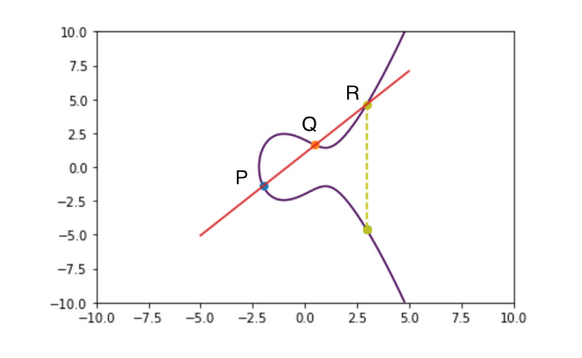
\includegraphics[width=\textwidth]{ECC.png}
	\caption{An elliptic curve. \cite{ECCbasics}}
\end{figure} 

\subsubsection{ECDSA} 
\label{subsubsec:ecdsa}

The elliptic curve digital signature algorithm (ECDSA) is the default elliptic curve variant of digital signatures. Like the standard digital signature algorithm (DSA), each signature with length $l$ guarantees a security level of $l/4$(e.g. a signature of 512 bits would guarantee a security level of 128 bits).

\subsubsection{ECDH} 
\label{subsubsec:ecdh}

Besides using ECC for digital signatures with ECDSA, another ECC based protocol that is chosen in this paper is elliptic curve Diffie-Hellman (ECDH). like normal Diffie-Hellman it is used when two communicating parties wish to establish a shared secret (or session key) over an insecure channel. First the two communication parties (Alice and Bob) agree on a base point $G$ and domain parameters $a$ and $b$ of the curve they will use. Second they both generate an ECC key pair: $(P_a,n_a)$ and $(P_b,n_b)$ where $P$ = $nG$ (the base point dotted with itself n times). Third they exchange their public keys $P_a$ and $P_b$. In the last step Alice calculates $S$ = $n_a P_b$ and Bob calculates $S$ = $n_b P_a$. It's important to note that $S$ is the same for both Alice and Bob since $S$ = $n_a P_b$ = $n_a ( n_b G )$ = $n_b ( n_a G )$ = $n_b P_a$. $S$ is the newly created session key that is shared by both parties. Any third party listening on the channel only knows $P_a$ and $P_b$, which are not enough to easily calculate $S$ since they would have to solve the ECDLP.

\subsubsection{ECDHE\_ECDSA} 
\label{subsubsec:ecdh_ecdsa}

As mentioned in section \ref{sec:AK} and illustrated in section \ref{sec:authentication_procedure} it is common practice to combine authentication and shared secret establishment into a single procedure. In \cite{RFC4492} multiple methods are proposed that perform ECDH, while also providing authentication using elliptic curve digital signatures. One of these methods is called ECDHE\_ECDSA and is illustrated in figure \ref{fig:ECDH2}. The extra E in ECDHE comes from th fact that this procedure uses "ephemeral" (i.e temporary) keys. Two communicating parties (Alice and Bob) are both in possession of an elliptic curve private/public key pair: $Pb_a$,$Pr_a$ (Alice) and $Pb_b$,$Pr_b$ (Bob). Alice signals to Bob that she wishes to initiate a ECDHE\_ECDSA sequence by sending a 'hello' message to Bob. Bob then creates a new ephemeral elliptic curve key pair: $Pb_{bE}$,$Pr_{bE}$, signs the new ephemeral public key using his own private key: Sig($Pb_{bE}$,$Pr_b$), and sends this to Alice. She will first verify the signature: Ver(Sig,$Pb_{b}$), thus authenticating Bob to Alice. After which she will also generate her own ephemeral key pair using the same curve as Bob: KGen($Pb_{aE}$,$Pr_{aE}$), before signing the new public key and sending it to Bob: Sig($Pb_{aE}$,$Pr_a$). Bob will then in turn verify the signature using Alice's public key: Ver(Sig,$Pb_{a}$). Alice and Bob are now both in possession resources (e.g. each others ephemeral public keys) to use ECDH to generate a shared secret: $K$=ECDH($Pr_{aE}$,$Pb_{bE}$) for Alice and $K$=ECDH($Pr_{bE}$,$Pb_{aE}$) for Bob. The attentive reader might wonder why these ephemeral key pairs are generated at all. why not use the pre-existing key pairs $Pb_a$,$Pr_a$ and $Pb_b$,$Pr_b$ to generate the shared secret. This is because introducing these ephemeral keys guarantees perfect forward secrecy (PFS)\footnote{Perfect forward secrecy is guaranteed when a posteriori leak of one of the used private keys (e.g. $Pr_a$ and $Pr_b$ in figure \ref{fig:ECDH2}) does not result in the communication session being compromised.}. This is because an attacker in possession of either $Pr_a$ or $Pr_b$ is still not able to obtain the shared secret.


\begin{figure}[h]
	\centering
	\fbox{
		\procedure{ECDHE\_ECDSA}{%
			\textbf{Alice}  \<\< \textbf{Bob} \\
			\text{$Pb_a$,$Pr_a$} \<\< \text{$Pb_b$,$Pr_b$} \\
			\< \sendmessageright{top=\text{hello}} \<\\
			\<\< \text{KGen($Pb_{bE}$,$Pr_{bE}$)} \\
			\< \sendmessageleft{top=\text{Sig($Pb_{bE}$,$Pr_b$)}} \<\\
			\text{Ver(Sig,$Pb_{b}$)} \<\< \\
			\text{KGen($Pb_{aE}$,$Pr_{aE}$)} \<\< \\
			\< \sendmessageright{top=\text{Sig($Pb_{aE}$,$Pr_a$)}} \<\\
			\<\< \text{Ver(Sig,$Pb_{a}$)} \\
			\text{$K$=ECDH($Pr_{aE}$,$Pb_{bE}$)} \<\< \text{$K$=ECDH($Pr_{bE}$,$Pb_{aE}$)} \\
		}
	}
	\caption{ECDHE\_ECDSA}
	\label{fig:ECDH2}
\end{figure} 

\subsection{SHA} 
\label{subsec:sha}

A lot of cryptographic procedures require the data to be hashed first, and the implementation of this research paper is certainly no exception. The choice was made to use the secure hash algorithm (SHA) family of hash functions. SHA constitutes a large set of cryptographic hash functions that were designed by the United States National Security Institute (NSA). There exist 4 distinct sets of SHA\cite{wiki:SHA}:

\begin{itemize}
	\item \textbf{SHA-0}: Published in 1993, was withdrawn shortly after publication because of a significant flaw.
	
	\item \textbf{SHA-1}: Published in 1995 as a replacement to SHA-0. Has been considered insufficiently secure since 2005.
	
	\item \textbf{SHA-2}: Published in 2001, consists of six hash functions with hash values that are 224, 256, 384 or 512 bits: SHA-224, SHA-256, SHA-384, SHA-512, SHA-512/224, SHA-512/256.
	
	\item \textbf{SHA-3}: Pubished in 2015, subset of the broader cryptographic primitive family Keccak. Conists of the following hash functions: SHA3-224, SHA3-256, SHA3-384 and SHA3-512.
\end{itemize} 
While the SHA-3 hash functions were an obvious candidate, simply because they are newer and deemed more secure, the choice was made to work with the HSA-2 hash functions instead. This is because secure SHA-2 libraries are more readily available for the architecture that was used in our implementation. Another reason is that the MAC function that was chosen also employs SHA-265 as it's cryptographic hash function. 

\subsection{HMAC} 
\label{subsec:hmac}

Once a session key is established between two parties this can be used to authenticate the messages they sent to each other. Since this configuration is symmetric, i.e. they both share the same secret, this is done by using a message authentication code (MAC). The choice was made to work with a hash-based message authentication code (HMAC). HMAC is a specific type of message authentication code (MAC) that uses a cryptographic hash function as well as a secret cryptographic key (in our case the session key established using ECDH). More specifically HMAC-265 (HMAC using SHA-265) was used since it sufficiently secure, as well as there being a library function readily available for our chosen architecture.